% Options for packages loaded elsewhere
\PassOptionsToPackage{unicode}{hyperref}
\PassOptionsToPackage{hyphens}{url}
%
\documentclass[
]{article}
\usepackage{lmodern}
\usepackage{amssymb,amsmath}
\usepackage{ifxetex,ifluatex}
\ifnum 0\ifxetex 1\fi\ifluatex 1\fi=0 % if pdftex
  \usepackage[T1]{fontenc}
  \usepackage[utf8]{inputenc}
  \usepackage{textcomp} % provide euro and other symbols
\else % if luatex or xetex
  \usepackage{unicode-math}
  \defaultfontfeatures{Scale=MatchLowercase}
  \defaultfontfeatures[\rmfamily]{Ligatures=TeX,Scale=1}
\fi
% Use upquote if available, for straight quotes in verbatim environments
\IfFileExists{upquote.sty}{\usepackage{upquote}}{}
\IfFileExists{microtype.sty}{% use microtype if available
  \usepackage[]{microtype}
  \UseMicrotypeSet[protrusion]{basicmath} % disable protrusion for tt fonts
}{}
\makeatletter
\@ifundefined{KOMAClassName}{% if non-KOMA class
  \IfFileExists{parskip.sty}{%
    \usepackage{parskip}
  }{% else
    \setlength{\parindent}{0pt}
    \setlength{\parskip}{6pt plus 2pt minus 1pt}}
}{% if KOMA class
  \KOMAoptions{parskip=half}}
\makeatother
\usepackage{xcolor}
\IfFileExists{xurl.sty}{\usepackage{xurl}}{} % add URL line breaks if available
\IfFileExists{bookmark.sty}{\usepackage{bookmark}}{\usepackage{hyperref}}
\hypersetup{
  pdftitle={Lab 3: Intro to Decision Theory},
  pdfauthor={Rebecca C. Steorts and Xingyu Yan},
  hidelinks,
  pdfcreator={LaTeX via pandoc}}
\urlstyle{same} % disable monospaced font for URLs
\usepackage[margin=1in]{geometry}
\usepackage{color}
\usepackage{fancyvrb}
\newcommand{\VerbBar}{|}
\newcommand{\VERB}{\Verb[commandchars=\\\{\}]}
\DefineVerbatimEnvironment{Highlighting}{Verbatim}{commandchars=\\\{\}}
% Add ',fontsize=\small' for more characters per line
\usepackage{framed}
\definecolor{shadecolor}{RGB}{248,248,248}
\newenvironment{Shaded}{\begin{snugshade}}{\end{snugshade}}
\newcommand{\AlertTok}[1]{\textcolor[rgb]{0.94,0.16,0.16}{#1}}
\newcommand{\AnnotationTok}[1]{\textcolor[rgb]{0.56,0.35,0.01}{\textbf{\textit{#1}}}}
\newcommand{\AttributeTok}[1]{\textcolor[rgb]{0.77,0.63,0.00}{#1}}
\newcommand{\BaseNTok}[1]{\textcolor[rgb]{0.00,0.00,0.81}{#1}}
\newcommand{\BuiltInTok}[1]{#1}
\newcommand{\CharTok}[1]{\textcolor[rgb]{0.31,0.60,0.02}{#1}}
\newcommand{\CommentTok}[1]{\textcolor[rgb]{0.56,0.35,0.01}{\textit{#1}}}
\newcommand{\CommentVarTok}[1]{\textcolor[rgb]{0.56,0.35,0.01}{\textbf{\textit{#1}}}}
\newcommand{\ConstantTok}[1]{\textcolor[rgb]{0.00,0.00,0.00}{#1}}
\newcommand{\ControlFlowTok}[1]{\textcolor[rgb]{0.13,0.29,0.53}{\textbf{#1}}}
\newcommand{\DataTypeTok}[1]{\textcolor[rgb]{0.13,0.29,0.53}{#1}}
\newcommand{\DecValTok}[1]{\textcolor[rgb]{0.00,0.00,0.81}{#1}}
\newcommand{\DocumentationTok}[1]{\textcolor[rgb]{0.56,0.35,0.01}{\textbf{\textit{#1}}}}
\newcommand{\ErrorTok}[1]{\textcolor[rgb]{0.64,0.00,0.00}{\textbf{#1}}}
\newcommand{\ExtensionTok}[1]{#1}
\newcommand{\FloatTok}[1]{\textcolor[rgb]{0.00,0.00,0.81}{#1}}
\newcommand{\FunctionTok}[1]{\textcolor[rgb]{0.00,0.00,0.00}{#1}}
\newcommand{\ImportTok}[1]{#1}
\newcommand{\InformationTok}[1]{\textcolor[rgb]{0.56,0.35,0.01}{\textbf{\textit{#1}}}}
\newcommand{\KeywordTok}[1]{\textcolor[rgb]{0.13,0.29,0.53}{\textbf{#1}}}
\newcommand{\NormalTok}[1]{#1}
\newcommand{\OperatorTok}[1]{\textcolor[rgb]{0.81,0.36,0.00}{\textbf{#1}}}
\newcommand{\OtherTok}[1]{\textcolor[rgb]{0.56,0.35,0.01}{#1}}
\newcommand{\PreprocessorTok}[1]{\textcolor[rgb]{0.56,0.35,0.01}{\textit{#1}}}
\newcommand{\RegionMarkerTok}[1]{#1}
\newcommand{\SpecialCharTok}[1]{\textcolor[rgb]{0.00,0.00,0.00}{#1}}
\newcommand{\SpecialStringTok}[1]{\textcolor[rgb]{0.31,0.60,0.02}{#1}}
\newcommand{\StringTok}[1]{\textcolor[rgb]{0.31,0.60,0.02}{#1}}
\newcommand{\VariableTok}[1]{\textcolor[rgb]{0.00,0.00,0.00}{#1}}
\newcommand{\VerbatimStringTok}[1]{\textcolor[rgb]{0.31,0.60,0.02}{#1}}
\newcommand{\WarningTok}[1]{\textcolor[rgb]{0.56,0.35,0.01}{\textbf{\textit{#1}}}}
\usepackage{graphicx,grffile}
\makeatletter
\def\maxwidth{\ifdim\Gin@nat@width>\linewidth\linewidth\else\Gin@nat@width\fi}
\def\maxheight{\ifdim\Gin@nat@height>\textheight\textheight\else\Gin@nat@height\fi}
\makeatother
% Scale images if necessary, so that they will not overflow the page
% margins by default, and it is still possible to overwrite the defaults
% using explicit options in \includegraphics[width, height, ...]{}
\setkeys{Gin}{width=\maxwidth,height=\maxheight,keepaspectratio}
% Set default figure placement to htbp
\makeatletter
\def\fps@figure{htbp}
\makeatother
\setlength{\emergencystretch}{3em} % prevent overfull lines
\providecommand{\tightlist}{%
  \setlength{\itemsep}{0pt}\setlength{\parskip}{0pt}}
\setcounter{secnumdepth}{-\maxdimen} % remove section numbering
% Custom definitions
% To use this customization file, insert the line "% Custom definitions
% To use this customization file, insert the line "% Custom definitions
% To use this customization file, insert the line "% Custom definitions
% To use this customization file, insert the line "\input{custom}" in the header of the tex file.

% Formatting

\tolerance=1000
\usepackage[margin=1in]{geometry}


% Packages

% \usepackage{amssymb,latexsym}
\usepackage{amssymb,amsfonts,amsmath,latexsym,amsthm}
\usepackage[usenames,dvipsnames]{color}
\usepackage[]{graphicx}
\usepackage[space]{grffile}
\usepackage{mathrsfs}   % fancy math font
% \usepackage[font=small,skip=0pt]{caption}
\usepackage[skip=0pt]{caption}
\usepackage{subcaption}
\usepackage{verbatim}
\usepackage{url}
\usepackage{bm}
\usepackage{dsfont}
\usepackage{extarrows}
\usepackage{multirow}
% \usepackage{wrapfig}
% \usepackage{epstopdf}
\usepackage{rotating}
\usepackage{tikz}
\usetikzlibrary{fit}					% fitting shapes to coordinates
%\usetikzlibrary{backgrounds}	% drawing the background after the foreground


% \usepackage[dvipdfm,colorlinks,citecolor=blue,linkcolor=blue,urlcolor=blue]{hyperref}
\usepackage[colorlinks,citecolor=blue,linkcolor=blue,urlcolor=blue]{hyperref}
%\usepackage{hyperref}
\usepackage[authoryear,round]{natbib}


%  Theorems, etc.

\theoremstyle{plain}
\newtheorem{theorem}{Theorem}[section]
\newtheorem{corollary}[theorem]{Corollary}
\newtheorem{lemma}[theorem]{Lemma}
\newtheorem{proposition}[theorem]{Proposition}
\newtheorem{condition}[theorem]{Condition}
% \newtheorem{conditions}[theorem]{Conditions}

\theoremstyle{definition}
\newtheorem{definition}[theorem]{Definition}
% \newtheorem*{unnumbered-definition}{Definition}
\newtheorem{example}[theorem]{Example}
\theoremstyle{remark}
\newtheorem*{remark}{Remark}
\numberwithin{equation}{section}




% Document-specific shortcuts
\newcommand{\btheta}{{\bm\theta}}
\newcommand{\bbtheta}{{\pmb{\bm\theta}}}

\newcommand{\commentary}[1]{\ifx\showcommentary\undefined\else \emph{#1}\fi}

\newcommand{\term}[1]{\textit{\textbf{#1}}}

% Math shortcuts

% Probability distributions
\DeclareMathOperator*{\Exp}{Exp}
\DeclareMathOperator*{\TExp}{TExp}
\DeclareMathOperator*{\Bernoulli}{Bernoulli}
\DeclareMathOperator*{\Beta}{Beta}
\DeclareMathOperator*{\Ga}{Gamma}
\DeclareMathOperator*{\TGamma}{TGamma}
\DeclareMathOperator*{\Poisson}{Poisson}
\DeclareMathOperator*{\Binomial}{Binomial}
\DeclareMathOperator*{\NormalGamma}{NormalGamma}
\DeclareMathOperator*{\InvGamma}{InvGamma}
\DeclareMathOperator*{\Cauchy}{Cauchy}
\DeclareMathOperator*{\Uniform}{Uniform}
\DeclareMathOperator*{\Gumbel}{Gumbel}
\DeclareMathOperator*{\Pareto}{Pareto}
\DeclareMathOperator*{\Mono}{Mono}
\DeclareMathOperator*{\Geometric}{Geometric}
\DeclareMathOperator*{\Wishart}{Wishart}

% Math operators
\DeclareMathOperator*{\argmin}{arg\,min}
\DeclareMathOperator*{\argmax}{arg\,max}
\DeclareMathOperator*{\Cov}{Cov}
\DeclareMathOperator*{\diag}{diag}
\DeclareMathOperator*{\median}{median}
\DeclareMathOperator*{\Vol}{Vol}

% Math characters
\newcommand{\R}{\mathbb{R}}
\newcommand{\Z}{\mathbb{Z}}
\newcommand{\E}{\mathbb{E}}
\renewcommand{\Pr}{\mathbb{P}}
\newcommand{\I}{\mathds{1}}
\newcommand{\V}{\mathbb{V}}

\newcommand{\A}{\mathcal{A}}
\newcommand{\C}{\mathcal{C}}
\newcommand{\D}{\mathcal{D}}
\newcommand{\Hcal}{\mathcal{H}}
\newcommand{\M}{\mathcal{M}}
\newcommand{\N}{\mathcal{N}}
\newcommand{\X}{\mathcal{X}}
\newcommand{\Zcal}{\mathcal{Z}}
\renewcommand{\P}{\mathcal{P}}

\newcommand{\T}{\mathtt{T}}
\renewcommand{\emptyset}{\varnothing}


% Miscellaneous commands
\newcommand{\iid}{\stackrel{\mathrm{iid}}{\sim}}
\newcommand{\matrixsmall}[1]{\bigl(\begin{smallmatrix}#1\end{smallmatrix} \bigr)}

\newcommand{\items}[1]{\begin{itemize} #1 \end{itemize}}

\newcommand{\todo}[1]{\emph{\textcolor{red}{(#1)}}}

\newcommand{\branch}[4]{
\left\{
	\begin{array}{ll}
		#1  & \mbox{if } #2 \\
		#3 & \mbox{if } #4
	\end{array}
\right.
}

% approximately proportional to
\def\app#1#2{%
  \mathrel{%
    \setbox0=\hbox{$#1\sim$}%
    \setbox2=\hbox{%
      \rlap{\hbox{$#1\propto$}}%
      \lower1.3\ht0\box0%
    }%
    \raise0.25\ht2\box2%
  }%
}
\def\approxprop{\mathpalette\app\relax}

% \newcommand{\approptoinn}[2]{\mathrel{\vcenter{
  % \offinterlineskip\halign{\hfil$##$\cr
    % #1\propto\cr\noalign{\kern2pt}#1\sim\cr\noalign{\kern-2pt}}}}}

% \newcommand{\approxpropto}{\mathpalette\approptoinn\relax}





" in the header of the tex file.

% Formatting

\tolerance=1000
\usepackage[margin=1in]{geometry}


% Packages

% \usepackage{amssymb,latexsym}
\usepackage{amssymb,amsfonts,amsmath,latexsym,amsthm}
\usepackage[usenames,dvipsnames]{color}
\usepackage[]{graphicx}
\usepackage[space]{grffile}
\usepackage{mathrsfs}   % fancy math font
% \usepackage[font=small,skip=0pt]{caption}
\usepackage[skip=0pt]{caption}
\usepackage{subcaption}
\usepackage{verbatim}
\usepackage{url}
\usepackage{bm}
\usepackage{dsfont}
\usepackage{extarrows}
\usepackage{multirow}
% \usepackage{wrapfig}
% \usepackage{epstopdf}
\usepackage{rotating}
\usepackage{tikz}
\usetikzlibrary{fit}					% fitting shapes to coordinates
%\usetikzlibrary{backgrounds}	% drawing the background after the foreground


% \usepackage[dvipdfm,colorlinks,citecolor=blue,linkcolor=blue,urlcolor=blue]{hyperref}
\usepackage[colorlinks,citecolor=blue,linkcolor=blue,urlcolor=blue]{hyperref}
%\usepackage{hyperref}
\usepackage[authoryear,round]{natbib}


%  Theorems, etc.

\theoremstyle{plain}
\newtheorem{theorem}{Theorem}[section]
\newtheorem{corollary}[theorem]{Corollary}
\newtheorem{lemma}[theorem]{Lemma}
\newtheorem{proposition}[theorem]{Proposition}
\newtheorem{condition}[theorem]{Condition}
% \newtheorem{conditions}[theorem]{Conditions}

\theoremstyle{definition}
\newtheorem{definition}[theorem]{Definition}
% \newtheorem*{unnumbered-definition}{Definition}
\newtheorem{example}[theorem]{Example}
\theoremstyle{remark}
\newtheorem*{remark}{Remark}
\numberwithin{equation}{section}




% Document-specific shortcuts
\newcommand{\btheta}{{\bm\theta}}
\newcommand{\bbtheta}{{\pmb{\bm\theta}}}

\newcommand{\commentary}[1]{\ifx\showcommentary\undefined\else \emph{#1}\fi}

\newcommand{\term}[1]{\textit{\textbf{#1}}}

% Math shortcuts

% Probability distributions
\DeclareMathOperator*{\Exp}{Exp}
\DeclareMathOperator*{\TExp}{TExp}
\DeclareMathOperator*{\Bernoulli}{Bernoulli}
\DeclareMathOperator*{\Beta}{Beta}
\DeclareMathOperator*{\Ga}{Gamma}
\DeclareMathOperator*{\TGamma}{TGamma}
\DeclareMathOperator*{\Poisson}{Poisson}
\DeclareMathOperator*{\Binomial}{Binomial}
\DeclareMathOperator*{\NormalGamma}{NormalGamma}
\DeclareMathOperator*{\InvGamma}{InvGamma}
\DeclareMathOperator*{\Cauchy}{Cauchy}
\DeclareMathOperator*{\Uniform}{Uniform}
\DeclareMathOperator*{\Gumbel}{Gumbel}
\DeclareMathOperator*{\Pareto}{Pareto}
\DeclareMathOperator*{\Mono}{Mono}
\DeclareMathOperator*{\Geometric}{Geometric}
\DeclareMathOperator*{\Wishart}{Wishart}

% Math operators
\DeclareMathOperator*{\argmin}{arg\,min}
\DeclareMathOperator*{\argmax}{arg\,max}
\DeclareMathOperator*{\Cov}{Cov}
\DeclareMathOperator*{\diag}{diag}
\DeclareMathOperator*{\median}{median}
\DeclareMathOperator*{\Vol}{Vol}

% Math characters
\newcommand{\R}{\mathbb{R}}
\newcommand{\Z}{\mathbb{Z}}
\newcommand{\E}{\mathbb{E}}
\renewcommand{\Pr}{\mathbb{P}}
\newcommand{\I}{\mathds{1}}
\newcommand{\V}{\mathbb{V}}

\newcommand{\A}{\mathcal{A}}
\newcommand{\C}{\mathcal{C}}
\newcommand{\D}{\mathcal{D}}
\newcommand{\Hcal}{\mathcal{H}}
\newcommand{\M}{\mathcal{M}}
\newcommand{\N}{\mathcal{N}}
\newcommand{\X}{\mathcal{X}}
\newcommand{\Zcal}{\mathcal{Z}}
\renewcommand{\P}{\mathcal{P}}

\newcommand{\T}{\mathtt{T}}
\renewcommand{\emptyset}{\varnothing}


% Miscellaneous commands
\newcommand{\iid}{\stackrel{\mathrm{iid}}{\sim}}
\newcommand{\matrixsmall}[1]{\bigl(\begin{smallmatrix}#1\end{smallmatrix} \bigr)}

\newcommand{\items}[1]{\begin{itemize} #1 \end{itemize}}

\newcommand{\todo}[1]{\emph{\textcolor{red}{(#1)}}}

\newcommand{\branch}[4]{
\left\{
	\begin{array}{ll}
		#1  & \mbox{if } #2 \\
		#3 & \mbox{if } #4
	\end{array}
\right.
}

% approximately proportional to
\def\app#1#2{%
  \mathrel{%
    \setbox0=\hbox{$#1\sim$}%
    \setbox2=\hbox{%
      \rlap{\hbox{$#1\propto$}}%
      \lower1.3\ht0\box0%
    }%
    \raise0.25\ht2\box2%
  }%
}
\def\approxprop{\mathpalette\app\relax}

% \newcommand{\approptoinn}[2]{\mathrel{\vcenter{
  % \offinterlineskip\halign{\hfil$##$\cr
    % #1\propto\cr\noalign{\kern2pt}#1\sim\cr\noalign{\kern-2pt}}}}}

% \newcommand{\approxpropto}{\mathpalette\approptoinn\relax}





" in the header of the tex file.

% Formatting

\tolerance=1000
\usepackage[margin=1in]{geometry}


% Packages

% \usepackage{amssymb,latexsym}
\usepackage{amssymb,amsfonts,amsmath,latexsym,amsthm}
\usepackage[usenames,dvipsnames]{color}
\usepackage[]{graphicx}
\usepackage[space]{grffile}
\usepackage{mathrsfs}   % fancy math font
% \usepackage[font=small,skip=0pt]{caption}
\usepackage[skip=0pt]{caption}
\usepackage{subcaption}
\usepackage{verbatim}
\usepackage{url}
\usepackage{bm}
\usepackage{dsfont}
\usepackage{extarrows}
\usepackage{multirow}
% \usepackage{wrapfig}
% \usepackage{epstopdf}
\usepackage{rotating}
\usepackage{tikz}
\usetikzlibrary{fit}					% fitting shapes to coordinates
%\usetikzlibrary{backgrounds}	% drawing the background after the foreground


% \usepackage[dvipdfm,colorlinks,citecolor=blue,linkcolor=blue,urlcolor=blue]{hyperref}
\usepackage[colorlinks,citecolor=blue,linkcolor=blue,urlcolor=blue]{hyperref}
%\usepackage{hyperref}
\usepackage[authoryear,round]{natbib}


%  Theorems, etc.

\theoremstyle{plain}
\newtheorem{theorem}{Theorem}[section]
\newtheorem{corollary}[theorem]{Corollary}
\newtheorem{lemma}[theorem]{Lemma}
\newtheorem{proposition}[theorem]{Proposition}
\newtheorem{condition}[theorem]{Condition}
% \newtheorem{conditions}[theorem]{Conditions}

\theoremstyle{definition}
\newtheorem{definition}[theorem]{Definition}
% \newtheorem*{unnumbered-definition}{Definition}
\newtheorem{example}[theorem]{Example}
\theoremstyle{remark}
\newtheorem*{remark}{Remark}
\numberwithin{equation}{section}




% Document-specific shortcuts
\newcommand{\btheta}{{\bm\theta}}
\newcommand{\bbtheta}{{\pmb{\bm\theta}}}

\newcommand{\commentary}[1]{\ifx\showcommentary\undefined\else \emph{#1}\fi}

\newcommand{\term}[1]{\textit{\textbf{#1}}}

% Math shortcuts

% Probability distributions
\DeclareMathOperator*{\Exp}{Exp}
\DeclareMathOperator*{\TExp}{TExp}
\DeclareMathOperator*{\Bernoulli}{Bernoulli}
\DeclareMathOperator*{\Beta}{Beta}
\DeclareMathOperator*{\Ga}{Gamma}
\DeclareMathOperator*{\TGamma}{TGamma}
\DeclareMathOperator*{\Poisson}{Poisson}
\DeclareMathOperator*{\Binomial}{Binomial}
\DeclareMathOperator*{\NormalGamma}{NormalGamma}
\DeclareMathOperator*{\InvGamma}{InvGamma}
\DeclareMathOperator*{\Cauchy}{Cauchy}
\DeclareMathOperator*{\Uniform}{Uniform}
\DeclareMathOperator*{\Gumbel}{Gumbel}
\DeclareMathOperator*{\Pareto}{Pareto}
\DeclareMathOperator*{\Mono}{Mono}
\DeclareMathOperator*{\Geometric}{Geometric}
\DeclareMathOperator*{\Wishart}{Wishart}

% Math operators
\DeclareMathOperator*{\argmin}{arg\,min}
\DeclareMathOperator*{\argmax}{arg\,max}
\DeclareMathOperator*{\Cov}{Cov}
\DeclareMathOperator*{\diag}{diag}
\DeclareMathOperator*{\median}{median}
\DeclareMathOperator*{\Vol}{Vol}

% Math characters
\newcommand{\R}{\mathbb{R}}
\newcommand{\Z}{\mathbb{Z}}
\newcommand{\E}{\mathbb{E}}
\renewcommand{\Pr}{\mathbb{P}}
\newcommand{\I}{\mathds{1}}
\newcommand{\V}{\mathbb{V}}

\newcommand{\A}{\mathcal{A}}
\newcommand{\C}{\mathcal{C}}
\newcommand{\D}{\mathcal{D}}
\newcommand{\Hcal}{\mathcal{H}}
\newcommand{\M}{\mathcal{M}}
\newcommand{\N}{\mathcal{N}}
\newcommand{\X}{\mathcal{X}}
\newcommand{\Zcal}{\mathcal{Z}}
\renewcommand{\P}{\mathcal{P}}

\newcommand{\T}{\mathtt{T}}
\renewcommand{\emptyset}{\varnothing}


% Miscellaneous commands
\newcommand{\iid}{\stackrel{\mathrm{iid}}{\sim}}
\newcommand{\matrixsmall}[1]{\bigl(\begin{smallmatrix}#1\end{smallmatrix} \bigr)}

\newcommand{\items}[1]{\begin{itemize} #1 \end{itemize}}

\newcommand{\todo}[1]{\emph{\textcolor{red}{(#1)}}}

\newcommand{\branch}[4]{
\left\{
	\begin{array}{ll}
		#1  & \mbox{if } #2 \\
		#3 & \mbox{if } #4
	\end{array}
\right.
}

% approximately proportional to
\def\app#1#2{%
  \mathrel{%
    \setbox0=\hbox{$#1\sim$}%
    \setbox2=\hbox{%
      \rlap{\hbox{$#1\propto$}}%
      \lower1.3\ht0\box0%
    }%
    \raise0.25\ht2\box2%
  }%
}
\def\approxprop{\mathpalette\app\relax}

% \newcommand{\approptoinn}[2]{\mathrel{\vcenter{
  % \offinterlineskip\halign{\hfil$##$\cr
    % #1\propto\cr\noalign{\kern2pt}#1\sim\cr\noalign{\kern-2pt}}}}}

% \newcommand{\approxpropto}{\mathpalette\approptoinn\relax}





" in the header of the tex file.

% Formatting

%\setbeamertemplate{navigation symbols}{}
%\setbeamertemplate{footline}[page number]


\usepackage{bbm}
% Packages
\usepackage{amssymb,amsfonts,amsmath,latexsym,amsthm}
%\usepackage[usenames,dvipsnames]{color}
%\usepackage[]{graphicx}
%\usepackage[space]{grffile}
\usepackage{mathrsfs} 
 \usepackage{amssymb,latexsym}
\usepackage{amssymb,amsfonts,amsmath,latexsym,amsthm, bm}
%\usepackage[usenames,dvipsnames]{color}
%\usepackage[]{graphicx}
%\usepackage[space]{grffile}
\usepackage{mathrsfs}   % fancy math font
% \usepackage[font=small,skip=0pt]{caption}
%\usepackage[skip=0pt]{caption}
%\usepackage{subcaption}
%\usepackage{verbatim}
%\usepackage{url}
%\usepackage{bm}
\usepackage{dsfont}
\usepackage{multirow}
%\usepackage{extarrows}
%\usepackage{multirow}
%% \usepackage{wrapfig}
%% \usepackage{epstopdf}
%\usepackage{rotating}
%\usepackage{tikz}
%\usetikzlibrary{fit}					% fitting shapes to coordinates
%\usetikzlibrary{backgrounds}	% drawing the background after the foreground


% \usepackage[dvipdfm,colorlinks,citecolor=blue,linkcolor=blue,urlcolor=blue]{hyperref}
%\usepackage[colorlinks,citecolor=blue,linkcolor=blue,urlcolor=blue]{hyperref}
%%\usepackage{hyperref}
%\usepackage[authoryear,round]{natbib}


%  Theorems, etc.

%\theoremstyle{plain}
%\newtheorem{theorem}{Theorem}[section]
%\newtheorem{corollary}[theorem]{Corollary}
%\newtheorem{lemma}[theorem]{Lemma}
%\newtheorem{proposition}[theorem]{Proposition}
%\newtheorem{condition}[theorem]{Condition}
% \newtheorem{conditions}[theorem]{Conditions}

%\theoremstyle{definition}
%\newtheorem{definition}[theorem]{Definition}
%% \newtheorem*{unnumbered-definition}{Definition}
%\newtheorem{example}[theorem]{Example}
%\theoremstyle{remark}
%\newtheorem*{remark}{Remark}
%\numberwithin{equation}{section}

\newcommand{\bz}   {\bm{z}}
\newcommand{\bY}   {\bm{Y}}

\newcommand{\hbeta}   {\hat{\beta}}
\newcommand{\hy}   {\hat{y}}


% Document-specific shortcuts
\newcommand{\btheta}{{\bm\theta}}
\newcommand{\bbtheta}{{\pmb{\bm\theta}}}

\newcommand{\commentary}[1]{\ifx\showcommentary\undefined\else \emph{#1}\fi}

\newcommand{\term}[1]{\textit{\textbf{#1}}}

% Math shortcuts

% Probability distributions
\DeclareMathOperator*{\Exp}{Exp}
\DeclareMathOperator*{\TExp}{TExp}
\DeclareMathOperator*{\Bernoulli}{Bernoulli}
\DeclareMathOperator*{\Beta}{Beta}
\DeclareMathOperator*{\Ga}{Gamma}
\DeclareMathOperator*{\TGamma}{TGamma}
\DeclareMathOperator*{\Poisson}{Poisson}
\DeclareMathOperator*{\Binomial}{Binomial}
\DeclareMathOperator*{\NormalGamma}{NormalGamma}
\DeclareMathOperator*{\InvGamma}{InvGamma}
\DeclareMathOperator*{\Cauchy}{Cauchy}
\DeclareMathOperator*{\Uniform}{Uniform}
\DeclareMathOperator*{\Gumbel}{Gumbel}
\DeclareMathOperator*{\Pareto}{Pareto}
\DeclareMathOperator*{\Mono}{Mono}
\DeclareMathOperator*{\Geometric}{Geometric}
\DeclareMathOperator*{\Wishart}{Wishart}

% Math operators
\DeclareMathOperator*{\argmin}{arg\,min}
\DeclareMathOperator*{\argmax}{arg\,max}
\DeclareMathOperator*{\Cov}{Cov}
\DeclareMathOperator*{\diag}{diag}
\DeclareMathOperator*{\median}{median}
\DeclareMathOperator*{\Vol}{Vol}

% Math characters
\newcommand{\R}{\mathbb{R}}
\newcommand{\Z}{\mathbb{Z}}
\newcommand{\E}{\mathbb{E}}
\renewcommand{\Pr}{\mathbb{P}}
\newcommand{\I}{\mathds{1}}
\newcommand{\V}{\mathbb{V}}
\newcommand{\bbeta}{\bm{\beta}}

\newcommand{\A}{\mathcal{A}}
%\newcommand{\C}{\mathcal{C}}
\newcommand{\D}{\mathcal{D}}
\newcommand{\Hcal}{\mathcal{H}}
\newcommand{\M}{\mathcal{M}}
\newcommand{\N}{\mathcal{N}}
\newcommand{\X}{\mathcal{X}}
\newcommand{\Zcal}{\mathcal{Z}}
\renewcommand{\P}{\mathcal{P}}


\newcommand{\T}{\mathtt{T}}
\renewcommand{\emptyset}{\varnothing}

\newcommand{\bmu}{\bm{\mu}}
\newcommand{\by}   {\bm{y}}
\newcommand{\bX}   {\bm{X}}
\newcommand{\sig}   {\Sigma}
\newcommand{\bx}{\ensuremath{\mathbf{x}}}
%\newcommand{\X}{\ensuremath{\mathbf{x}}}
%\newcommand{\w}{\ensuremath{\mathbf{w}}}
%\newcommand{\h}{\ensuremath{\mathbf{h}}}
%\newcommand{\V}{\ensuremath{\mathbf{v}}}
%\newcommand{\cov}{\text{Cov}}
\newcommand{\var}{\text{Var}}
\newcommand{\Var}{\text{Var}}



% Miscellaneous commands
\newcommand{\iid}{\stackrel{\mathrm{iid}}{\sim}}
\newcommand{\matrixsmall}[1]{\bigl(\begin{smallmatrix}#1\end{smallmatrix} \bigr)}

\newcommand{\items}[1]{\begin{itemize} #1 \end{itemize}}

\newcommand{\todo}[1]{\emph{\textcolor{red}{(#1)}}}

\newcommand{\branch}[4]{
\left\{
	\begin{array}{ll}
		#1  & \mbox{if } #2 \\
		#3 & \mbox{if } #4
	\end{array}
\right.
}

% approximately proportional to
\def\app#1#2{%
  \mathrel{%
    \setbox0=\hbox{$#1\sim$}%
    \setbox2=\hbox{%
      \rlap{\hbox{$#1\propto$}}%
      \lower1.3\ht0\box0%
    }%
    \raise0.25\ht2\box2%
  }%
}
\def\approxprop{\mathpalette\app\relax}

% \newcommand{\approptoinn}[2]{\mathrel{\vcenter{
  % \offinterlineskip\halign{\hfil$##$\cr
    % #1\propto\cr\noalign{\kern2pt}#1\sim\cr\noalign{\kern-2pt}}}}}

% \newcommand{\approxpropto}{\mathpalette\approptoinn\relax}

\title{Lab 3: Intro to Decision Theory}
\author{Rebecca C. Steorts and Xingyu Yan}
\date{}

\begin{document}
\maketitle

In class, you saw the resource allocation example. We will now go
through how to reproduce parts of the lecture using R for all the tasks.
While these will not be part of your weekly homework assignment, please
do work on it on your own to make sure that you have an understanding of
it.

Let's briefly recall the problem statement and set up that we saw in
class.

Suppose public health officials in a small city need to decide how much
resources to devote toward prevention and treatment of a certain
disease, but the fraction \(\theta\) of infected individuals in the city
is unknown.

Suppose they allocate enough resources to accomodate a fraction \(c\) of
the population. If \(c\) is too large, there will be wasted resources,
while if it is too small, preventable cases may occur and some
individuals may go untreated. After deliberation, they tentatively adopt
the following loss function:

\[\ell(\theta,c) =\branch{|\theta-c|}{c\geq\theta}
                       {10|\theta-c|}{c<\theta.}\]

By considering data from other similar cities, they determine a prior
\(p(\theta)\).

For simplicity, suppose \[\theta \sim \Beta(a,b)\] (i.e.,
\(p(\theta) = \Beta(\theta|a,b)\)), with \(a=0.05\) and \(b=1\).

They conduct a survey assessing the disease status of \(n=30\)
individuals, \(x_1,\ldots,x_n\). This is modeled as
\[X_1,\ldots,X_n \stackrel{iid}{\sim} \Bernoulli(\theta),\] which is
reasonable if the individuals are uniformly sampled and the population
is large. Suppose all but one are disease-free, i.e.,
\(\sum_{i=1}^n x_i = 1\).

\hypertarget{summary-of-tasks}{%
\section{Summary of Tasks}\label{summary-of-tasks}}

\begin{enumerate}
\def\labelenumi{\arabic{enumi}.}
\tightlist
\item
  We know \(p(\theta|x)\) as an updated Beta, so we can numerically
  compute this integral for each \(c\). Reproduce Figure 1 from lecture,
  illustrating \(\rho(c,x)\) for our example. Also, work through where
  the minimum occurs numerically (\(c\approx 0.08\)).
\item
  Now perform a sensitivity analysis for the prior assumption
  (Beta(a,b)). What do you find?
\item
  Consider the Bayes procedure (\(c\approx 0.08\)),
  \(c=\bar{x}, c=0.1.\)
\item
  Plot the frequentist risk \(R(\theta, \delta)\) as a function of
  \(\theta\) for the three procedures in the previous task. Report your
  findings.
\item
  Based on your plot of the frequentist risk, consider the three
  estimators---the constant, the mean, and the Bayes estimators. Which
  estimators are admissible? Be sure to explain why or why they are not
  admissible.
\end{enumerate}

\hypertarget{task-1}{%
\section{Task 1}\label{task-1}}

Reproduce Figure 1 from lecture, illustrating \(\rho(c,x)\) for our
example. Also, work through where the minimum occurs numerically
(\(c\approx 0.08\)).

Solution:

\begin{Shaded}
\begin{Highlighting}[]
\CommentTok{# set seed }
\KeywordTok{set.seed}\NormalTok{(}\DecValTok{123}\NormalTok{)}

\CommentTok{# data}
\NormalTok{sum_x =}\StringTok{ }\DecValTok{1}
\NormalTok{n =}\StringTok{ }\DecValTok{30}
\CommentTok{# prior parameters}
\NormalTok{a =}\StringTok{ }\FloatTok{0.05}\NormalTok{; b =}\StringTok{ }\DecValTok{1}
\CommentTok{# posterior parameters}
\NormalTok{an =}\StringTok{ }\NormalTok{a }\OperatorTok{+}\StringTok{ }\NormalTok{sum_x}
\NormalTok{bn =}\StringTok{ }\NormalTok{b }\OperatorTok{+}\StringTok{ }\NormalTok{n }\OperatorTok{-}\StringTok{ }\NormalTok{sum_x}
\NormalTok{th =}\StringTok{ }\KeywordTok{seq}\NormalTok{(}\DecValTok{0}\NormalTok{,}\DecValTok{1}\NormalTok{,}\DataTypeTok{length.out =} \DecValTok{100}\NormalTok{)}
\NormalTok{like =}\StringTok{ }\KeywordTok{dbeta}\NormalTok{(th, sum_x}\OperatorTok{+}\DecValTok{1}\NormalTok{,n}\OperatorTok{-}\NormalTok{sum_x}\OperatorTok{+}\DecValTok{1}\NormalTok{)}
\NormalTok{prior =}\StringTok{ }\KeywordTok{dbeta}\NormalTok{(th,a,b)}
\NormalTok{post =}\StringTok{ }\KeywordTok{dbeta}\NormalTok{(th,sum_x}\OperatorTok{+}\NormalTok{a,n}\OperatorTok{-}\NormalTok{sum_x}\OperatorTok{+}\NormalTok{b)}
\end{Highlighting}
\end{Shaded}

We now consider the loss function.

\begin{Shaded}
\begin{Highlighting}[]
\CommentTok{# compute the loss given theta and c }
\NormalTok{loss_function =}\StringTok{ }\ControlFlowTok{function}\NormalTok{(theta, c)\{}
  \ControlFlowTok{if}\NormalTok{ (c }\OperatorTok{<}\StringTok{ }\NormalTok{theta)\{}
    \KeywordTok{return}\NormalTok{(}\DecValTok{10}\OperatorTok{*}\KeywordTok{abs}\NormalTok{(theta }\OperatorTok{-}\StringTok{ }\NormalTok{c))}
\NormalTok{  \} }\ControlFlowTok{else}\NormalTok{\{}
    \KeywordTok{return}\NormalTok{(}\DataTypeTok{l =} \KeywordTok{abs}\NormalTok{(theta }\OperatorTok{-}\StringTok{ }\NormalTok{c))}
\NormalTok{  \}}
\NormalTok{\}}
\end{Highlighting}
\end{Shaded}

We now write a function \textbf{posterior\_risk} which is a function of
c, parameters a\_prior and b\_prior for the prior distribution of
\(\theta\), the summation of \(x_i\) sum\_x, the number of observations
n, and also the number of random draws s.

\begin{Shaded}
\begin{Highlighting}[]
\CommentTok{# compute the posterior risk given c }
\CommentTok{# s is the number of random draws }
\NormalTok{posterior_risk =}\StringTok{ }\ControlFlowTok{function}\NormalTok{(c, a_prior, b_prior, sum_x, n, }\DataTypeTok{s =} \DecValTok{30000}\NormalTok{)\{}
  \CommentTok{# randow draws from beta distribution }
\NormalTok{  a_post =}\StringTok{ }\NormalTok{a_prior }\OperatorTok{+}\StringTok{ }\NormalTok{sum_x}
\NormalTok{  b_post =}\StringTok{ }\NormalTok{b_prior }\OperatorTok{+}\StringTok{ }\NormalTok{n }\OperatorTok{-}\StringTok{ }\NormalTok{sum_x}
\NormalTok{  theta =}\StringTok{ }\KeywordTok{rbeta}\NormalTok{(s, a_post, b_post)}
\NormalTok{  loss <-}\StringTok{ }\KeywordTok{apply}\NormalTok{(}\KeywordTok{as.matrix}\NormalTok{(theta),}\DecValTok{1}\NormalTok{,loss_function,c)}
  \CommentTok{# average values from the loss function}
\NormalTok{  risk =}\StringTok{ }\KeywordTok{mean}\NormalTok{(loss)}
\NormalTok{\}}
\CommentTok{# a sequence of c in [0, 0.5]}
\NormalTok{c =}\StringTok{ }\KeywordTok{seq}\NormalTok{(}\DecValTok{0}\NormalTok{, }\FloatTok{0.5}\NormalTok{, }\DataTypeTok{by =} \FloatTok{0.01}\NormalTok{)}
\NormalTok{post_risk <-}\StringTok{ }\KeywordTok{apply}\NormalTok{(}\KeywordTok{as.matrix}\NormalTok{(c),}\DecValTok{1}\NormalTok{,posterior_risk, a, b, sum_x, n)}
\KeywordTok{head}\NormalTok{(post_risk)}
\end{Highlighting}
\end{Shaded}

\begin{verbatim}
## [1] 0.33917940 0.25367603 0.18868962 0.14489894 0.11693106 0.09453471
\end{verbatim}

We then look at the Posterior expected loss (posterior risk) for disease
prevelance versus c.~

\begin{Shaded}
\begin{Highlighting}[]
\CommentTok{# plot posterior risk against c }
\KeywordTok{plot}\NormalTok{(c, post_risk, }\DataTypeTok{type =} \StringTok{'l'}\NormalTok{, }\DataTypeTok{col=}\StringTok{'blue'}\NormalTok{, }
    \DataTypeTok{lwd =} \DecValTok{3}\NormalTok{, }\DataTypeTok{ylab =}\StringTok{'p(c, x)'}\NormalTok{ )}
\end{Highlighting}
\end{Shaded}

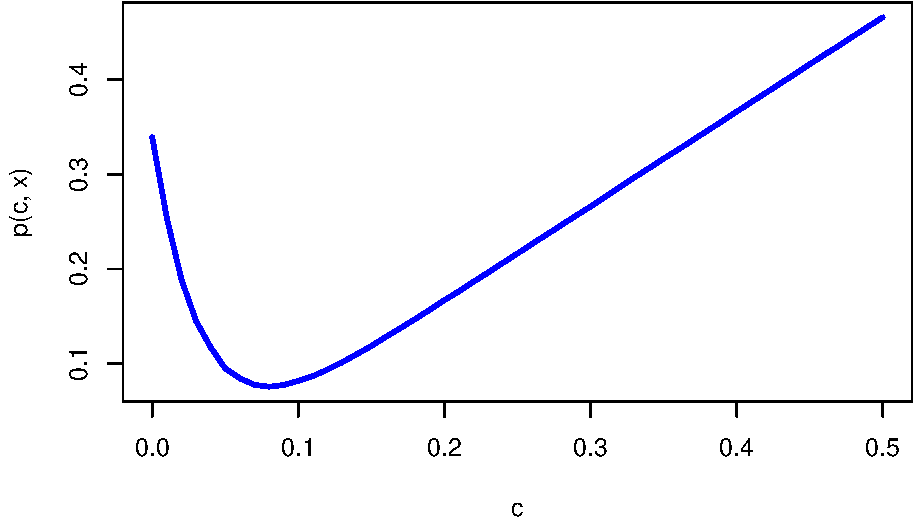
\includegraphics{lab-03_files/figure-latex/unnamed-chunk-4-1.pdf}

\begin{Shaded}
\begin{Highlighting}[]
\CommentTok{# minimum of posterior risk occurs at c = 0.08}
\NormalTok{(c[}\KeywordTok{which.min}\NormalTok{(post_risk)])}
\end{Highlighting}
\end{Shaded}

\begin{verbatim}
## [1] 0.08
\end{verbatim}

We have reproduced Figure 1, and shown that the minimum of posterior
risk occurs at \(c = 0.08.\)

\hypertarget{task-2}{%
\section{Task 2}\label{task-2}}

Now we perform a sensitivity analysis for the prior assumption on
\(\theta\).

We set \(a = 0.05, 1, 0.05\) and \(b = 1, 2, 10\).

If we have different values of \(a,b\), the posterior risk is minimized
at different values of \(c\). The optimal c depends on not only the
data, but also the prior setting.

\begin{Shaded}
\begin{Highlighting}[]
\CommentTok{# set prior}
\NormalTok{as =}\StringTok{ }\KeywordTok{c}\NormalTok{(}\FloatTok{0.05}\NormalTok{, }\DecValTok{1}\NormalTok{, }\FloatTok{0.05}\NormalTok{); bs =}\StringTok{ }\KeywordTok{c}\NormalTok{(}\DecValTok{1}\NormalTok{, }\DecValTok{1}\NormalTok{, }\DecValTok{10}\NormalTok{)}
\CommentTok{# initialize posterior risk}
\NormalTok{post_risk =}\StringTok{ }\KeywordTok{matrix}\NormalTok{(}\OtherTok{NA}\NormalTok{, }\DecValTok{3}\NormalTok{, }\KeywordTok{length}\NormalTok{(c))}

\CommentTok{# for each pair of a and b, compute the posterior risks}
\ControlFlowTok{for}\NormalTok{ (i }\ControlFlowTok{in} \DecValTok{1}\OperatorTok{:}\DecValTok{3}\NormalTok{)\{}
\NormalTok{  a_prior =}\StringTok{ }\NormalTok{as[i]}
\NormalTok{  b_prior =}\StringTok{ }\NormalTok{bs[i]}
  
\NormalTok{  post_risk[i,] =}\StringTok{ }\KeywordTok{apply}\NormalTok{(}\KeywordTok{as.matrix}\NormalTok{(c), }\DecValTok{1}\NormalTok{, posterior_risk, a_prior, b_prior, sum_x, n)}
\NormalTok{\}}

\CommentTok{# plot the posterior risk (for each prior setting)}
\KeywordTok{plot}\NormalTok{(c, post_risk[}\DecValTok{1}\NormalTok{,], }\DataTypeTok{type =} \StringTok{'l'}\NormalTok{, }\DataTypeTok{col=}\StringTok{'blue'}\NormalTok{, }\DataTypeTok{lty =} \DecValTok{1}\NormalTok{, }\DataTypeTok{yaxt =} \StringTok{"n"}\NormalTok{, }\DataTypeTok{ylab =} \StringTok{"p(c, x)"}\NormalTok{)}
\KeywordTok{par}\NormalTok{(}\DataTypeTok{new =}\NormalTok{ T)}
\KeywordTok{plot}\NormalTok{(c, post_risk[}\DecValTok{2}\NormalTok{,], }\DataTypeTok{type =} \StringTok{'l'}\NormalTok{, }\DataTypeTok{col=}\StringTok{'red'}\NormalTok{, }\DataTypeTok{lty =} \DecValTok{2}\NormalTok{, }\DataTypeTok{yaxt =} \StringTok{"n"}\NormalTok{, }\DataTypeTok{ylab =} \StringTok{""}\NormalTok{)}
\KeywordTok{par}\NormalTok{(}\DataTypeTok{new =}\NormalTok{ T)}
\KeywordTok{plot}\NormalTok{(c, post_risk[}\DecValTok{3}\NormalTok{,], }\DataTypeTok{type =} \StringTok{'l'}\NormalTok{, }\DataTypeTok{lty =} \DecValTok{3}\NormalTok{, }\DataTypeTok{yaxt =} \StringTok{"n"}\NormalTok{, }\DataTypeTok{ylab =} \StringTok{""}\NormalTok{)}
\KeywordTok{legend}\NormalTok{(}\StringTok{"bottomright"}\NormalTok{, }\DataTypeTok{lty =} \KeywordTok{c}\NormalTok{(}\DecValTok{1}\NormalTok{,}\DecValTok{2}\NormalTok{,}\DecValTok{3}\NormalTok{), }\DataTypeTok{col =} \KeywordTok{c}\NormalTok{(}\StringTok{"blue"}\NormalTok{, }\StringTok{"red"}\NormalTok{, }\StringTok{"black"}\NormalTok{), }
       \DataTypeTok{legend =} \KeywordTok{c}\NormalTok{(}\StringTok{"a = 0.05 b = 1"}\NormalTok{, }\StringTok{"a = 1 b = 1"}\NormalTok{, }\StringTok{"a = 0.05 b = 5"}\NormalTok{))}
\end{Highlighting}
\end{Shaded}

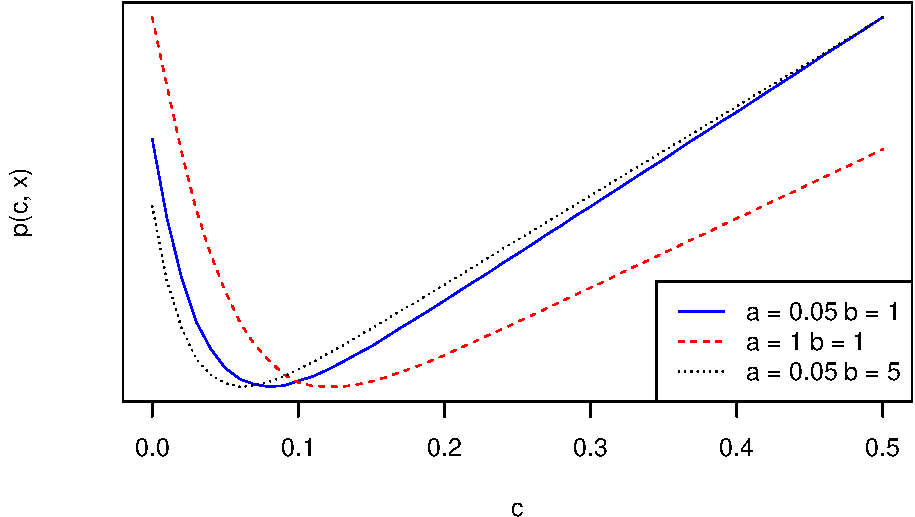
\includegraphics{lab-03_files/figure-latex/unnamed-chunk-5-1.pdf}

Remark: There is a more automated solution but this is one of most
simple solutions and is completely correct.

\hypertarget{task-3}{%
\section{Task 3}\label{task-3}}

Consider the Bayes procedure (\(c\approx 0.08\)), \(c=\bar{x}, c=0.1.\)
Reproduce Figure 2. Explain your findings.

The Bayes procedure always picks c to be a little bigger than
\(\bar{x}\).

\begin{Shaded}
\begin{Highlighting}[]
\CommentTok{# find the sum of the x's}
\NormalTok{sum_xs =}\StringTok{ }\KeywordTok{seq}\NormalTok{(}\DecValTok{0}\NormalTok{, }\DecValTok{30}\NormalTok{)}
\CommentTok{# initialize the minimum c}
\NormalTok{min_c =}\StringTok{ }\KeywordTok{matrix}\NormalTok{(}\OtherTok{NA}\NormalTok{, }\DecValTok{3}\NormalTok{, }\KeywordTok{length}\NormalTok{(sum_xs))}

\CommentTok{# find_optimal_C finds the optimal c under the Bayes procedure}
\CommentTok{# function of sum of x, parameters for prior, number of observations, and number of random draws }
\NormalTok{find_optimal_C <-}\StringTok{ }\ControlFlowTok{function}\NormalTok{(sum_x, a_prior, b_prior, n, }\DataTypeTok{s =} \DecValTok{500}\NormalTok{)\{}
\NormalTok{  c =}\StringTok{ }\KeywordTok{seq}\NormalTok{(}\DecValTok{0}\NormalTok{, }\DecValTok{1}\NormalTok{, }\DataTypeTok{by =} \FloatTok{0.01}\NormalTok{)}
\NormalTok{  post_risk =}\StringTok{  }\KeywordTok{apply}\NormalTok{(}\KeywordTok{as.matrix}\NormalTok{(c), }\DecValTok{1}\NormalTok{, posterior_risk, a_prior, b_prior, sum_x, n, s)}
\NormalTok{  c[}\KeywordTok{which.min}\NormalTok{(post_risk)]}
\NormalTok{\}}

\NormalTok{min_c[}\DecValTok{1}\NormalTok{,] =}\StringTok{ }\KeywordTok{apply}\NormalTok{(}\KeywordTok{as.matrix}\NormalTok{(sum_xs), }\DecValTok{1}\NormalTok{, find_optimal_C, a, b, n)}
\CommentTok{# find optimal c under sample mean}
\NormalTok{min_c[}\DecValTok{2}\NormalTok{,] =}\StringTok{ }\NormalTok{(sum_xs)}\OperatorTok{/}\NormalTok{n}
\CommentTok{# constant c }
\NormalTok{min_c[}\DecValTok{3}\NormalTok{,] =}\StringTok{ }\FloatTok{0.1}

\CommentTok{# plot Bayes procedure, sample mean, and constant }
\KeywordTok{plot}\NormalTok{(sum_xs, min_c[}\DecValTok{1}\NormalTok{,], }\DataTypeTok{col=}\StringTok{'blue'}\NormalTok{,}\DataTypeTok{type =} \StringTok{'o'}\NormalTok{,}\DataTypeTok{pch =} \DecValTok{16}\NormalTok{, }
     \DataTypeTok{ylab =} \StringTok{"resources allocated"}\NormalTok{, }\DataTypeTok{xlab =} \StringTok{'observed number of diseased cases'}\NormalTok{,}
     \DataTypeTok{ylim =} \KeywordTok{c}\NormalTok{(}\DecValTok{0}\NormalTok{,}\DecValTok{1}\NormalTok{))}
\KeywordTok{par}\NormalTok{(}\DataTypeTok{new =}\NormalTok{ T)}
\KeywordTok{plot}\NormalTok{(sum_xs, min_c[}\DecValTok{2}\NormalTok{,], }\DataTypeTok{type =} \StringTok{'o'}\NormalTok{, }\DataTypeTok{col=}\StringTok{'green'}\NormalTok{, }
     \DataTypeTok{pch =} \DecValTok{16}\NormalTok{, }\DataTypeTok{ylab =} \StringTok{""}\NormalTok{, }\DataTypeTok{xlab =} \StringTok{''}\NormalTok{, }\DataTypeTok{ylim =} \KeywordTok{c}\NormalTok{(}\DecValTok{0}\NormalTok{,}\DecValTok{1}\NormalTok{))}
\KeywordTok{par}\NormalTok{(}\DataTypeTok{new =}\NormalTok{ T)}
\KeywordTok{plot}\NormalTok{(sum_xs, min_c[}\DecValTok{3}\NormalTok{,], }\DataTypeTok{type =} \StringTok{'o'}\NormalTok{,}\DataTypeTok{col =} \StringTok{'red'}\NormalTok{,}
     \DataTypeTok{pch =} \DecValTok{16}\NormalTok{, }\DataTypeTok{ylab =} \StringTok{""}\NormalTok{, }\DataTypeTok{xlab =} \StringTok{''}\NormalTok{, }\DataTypeTok{ylim =} \KeywordTok{c}\NormalTok{(}\DecValTok{0}\NormalTok{,}\DecValTok{1}\NormalTok{))}
\KeywordTok{legend}\NormalTok{(}\StringTok{"topleft"}\NormalTok{, }\DataTypeTok{lty =} \KeywordTok{c}\NormalTok{(}\DecValTok{1}\NormalTok{,}\DecValTok{1}\NormalTok{,}\DecValTok{1}\NormalTok{), }\DataTypeTok{pch =} \KeywordTok{c}\NormalTok{(}\DecValTok{16}\NormalTok{,}\DecValTok{16}\NormalTok{,}\DecValTok{16}\NormalTok{),}
       \DataTypeTok{col =} \KeywordTok{c}\NormalTok{(}\StringTok{"blue"}\NormalTok{, }\StringTok{"green"}\NormalTok{, }\StringTok{"red"}\NormalTok{),}
       \DataTypeTok{legend =} \KeywordTok{c}\NormalTok{(}\StringTok{"Bayes"}\NormalTok{, }\StringTok{"Sample mean"}\NormalTok{, }\StringTok{"constant"}\NormalTok{))}
\end{Highlighting}
\end{Shaded}

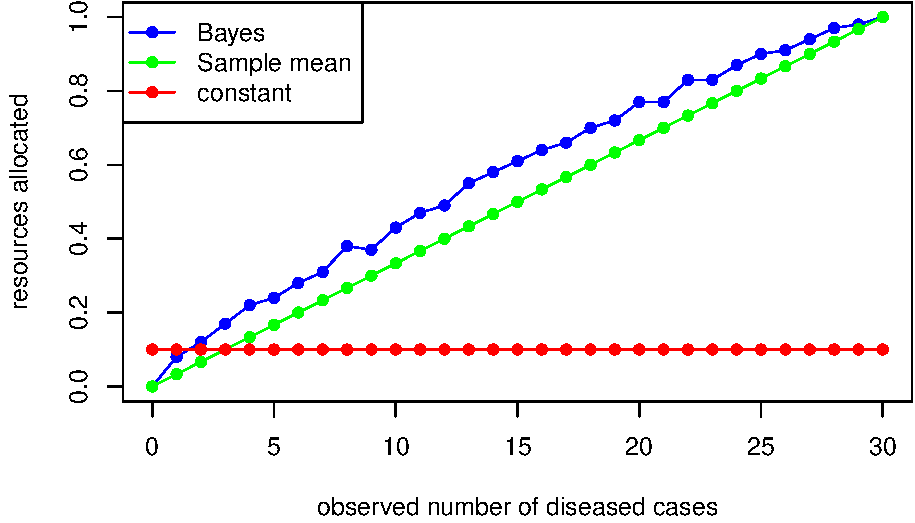
\includegraphics{lab-03_files/figure-latex/unnamed-chunk-6-1.pdf}

\hypertarget{task-4}{%
\section{Task 4}\label{task-4}}

For all \(\theta\), the Bayes procedure has the lower frequentist risk
than the sample mean.

\begin{Shaded}
\begin{Highlighting}[]
\NormalTok{thetas =}\StringTok{ }\KeywordTok{seq}\NormalTok{(}\DecValTok{0}\NormalTok{, }\DecValTok{1}\NormalTok{, }\DataTypeTok{by=}\FloatTok{0.1}\NormalTok{)}

\CommentTok{# frequentist risk for the 3 estimators given a theta}
\NormalTok{frequentist_risk =}\StringTok{ }\ControlFlowTok{function}\NormalTok{(theta)\{}
\NormalTok{  sum_xs =}\StringTok{ }\KeywordTok{rbinom}\NormalTok{(}\DecValTok{100}\NormalTok{, }\DecValTok{30}\NormalTok{, theta)}
\NormalTok{  Bayes_optimal =}\StringTok{ }\KeywordTok{apply}\NormalTok{(}\KeywordTok{as.matrix}\NormalTok{(sum_xs), }\DecValTok{1}\NormalTok{, find_optimal_C, a, b, n, }\DataTypeTok{s =} \DecValTok{100}\NormalTok{)}
\NormalTok{  mean_c =}\StringTok{ }\NormalTok{sum_xs }\OperatorTok{/}\StringTok{ }\DecValTok{30}
  
\NormalTok{  loss1 =}\StringTok{ }\KeywordTok{apply}\NormalTok{(}\KeywordTok{as.matrix}\NormalTok{(Bayes_optimal), }\DecValTok{1}\NormalTok{, loss_function, }\DataTypeTok{theta =}\NormalTok{ theta)}
\NormalTok{  loss2 =}\StringTok{ }\KeywordTok{apply}\NormalTok{(}\KeywordTok{as.matrix}\NormalTok{(mean_c), }\DecValTok{1}\NormalTok{, loss_function, }\DataTypeTok{theta =}\NormalTok{ theta )}
\NormalTok{  risk1 =}\StringTok{ }\KeywordTok{mean}\NormalTok{(loss1)}
\NormalTok{  risk2 =}\StringTok{ }\KeywordTok{mean}\NormalTok{(loss2)}
\NormalTok{  risk3 =}\StringTok{ }\KeywordTok{loss_function}\NormalTok{(theta, }\FloatTok{0.1}\NormalTok{)}
  \KeywordTok{return}\NormalTok{(}\KeywordTok{c}\NormalTok{(risk1, risk2, risk3))}
\NormalTok{\}}

\CommentTok{# given a sequance a theta, compute frequentist risk for each theta}
\NormalTok{R =}\StringTok{ }\KeywordTok{apply}\NormalTok{(}\KeywordTok{as.matrix}\NormalTok{(thetas), }\DecValTok{1}\NormalTok{, frequentist_risk)}

\CommentTok{# plot}
\KeywordTok{plot}\NormalTok{(thetas, R[}\DecValTok{1}\NormalTok{,], }\DataTypeTok{col=}\StringTok{'blue'}\NormalTok{, }\DataTypeTok{type =} \StringTok{"l"}\NormalTok{, }
     \DataTypeTok{ylab =} \StringTok{"frequentist risk"}\NormalTok{, }\DataTypeTok{xlab =} \StringTok{'theta'}\NormalTok{,}\DataTypeTok{ylim =} \KeywordTok{c}\NormalTok{(}\DecValTok{0}\NormalTok{,}\DecValTok{1}\NormalTok{))}
\KeywordTok{par}\NormalTok{(}\DataTypeTok{new =}\NormalTok{ T)}
\KeywordTok{plot}\NormalTok{(thetas, R[}\DecValTok{2}\NormalTok{,], }\DataTypeTok{type =} \StringTok{'l'}\NormalTok{, }\DataTypeTok{col=}\StringTok{'green'}\NormalTok{, }
     \DataTypeTok{ylab =} \StringTok{""}\NormalTok{, }\DataTypeTok{xlab =} \StringTok{''}\NormalTok{, }\DataTypeTok{ylim =} \KeywordTok{c}\NormalTok{(}\DecValTok{0}\NormalTok{,}\DecValTok{1}\NormalTok{))}
\KeywordTok{par}\NormalTok{(}\DataTypeTok{new =}\NormalTok{ T)}
\KeywordTok{plot}\NormalTok{(thetas, R[}\DecValTok{3}\NormalTok{,], }\DataTypeTok{type =} \StringTok{'l'}\NormalTok{,}\DataTypeTok{col =} \StringTok{'red'}\NormalTok{,}
     \DataTypeTok{ylab =} \StringTok{""}\NormalTok{, }\DataTypeTok{xlab =} \StringTok{''}\NormalTok{, }\DataTypeTok{ylim =} \KeywordTok{c}\NormalTok{(}\DecValTok{0}\NormalTok{,}\DecValTok{1}\NormalTok{))}
\KeywordTok{legend}\NormalTok{(}\StringTok{"topright"}\NormalTok{, }\DataTypeTok{lty =} \KeywordTok{c}\NormalTok{(}\DecValTok{1}\NormalTok{,}\DecValTok{1}\NormalTok{,}\DecValTok{1}\NormalTok{), }\DataTypeTok{col =} \KeywordTok{c}\NormalTok{(}\StringTok{"blue"}\NormalTok{, }\StringTok{"green"}\NormalTok{, }\StringTok{"red"}\NormalTok{),}
       \DataTypeTok{legend =} \KeywordTok{c}\NormalTok{(}\StringTok{"Bayes"}\NormalTok{, }\StringTok{"Sample mean"}\NormalTok{, }\StringTok{"constant"}\NormalTok{))}
\end{Highlighting}
\end{Shaded}

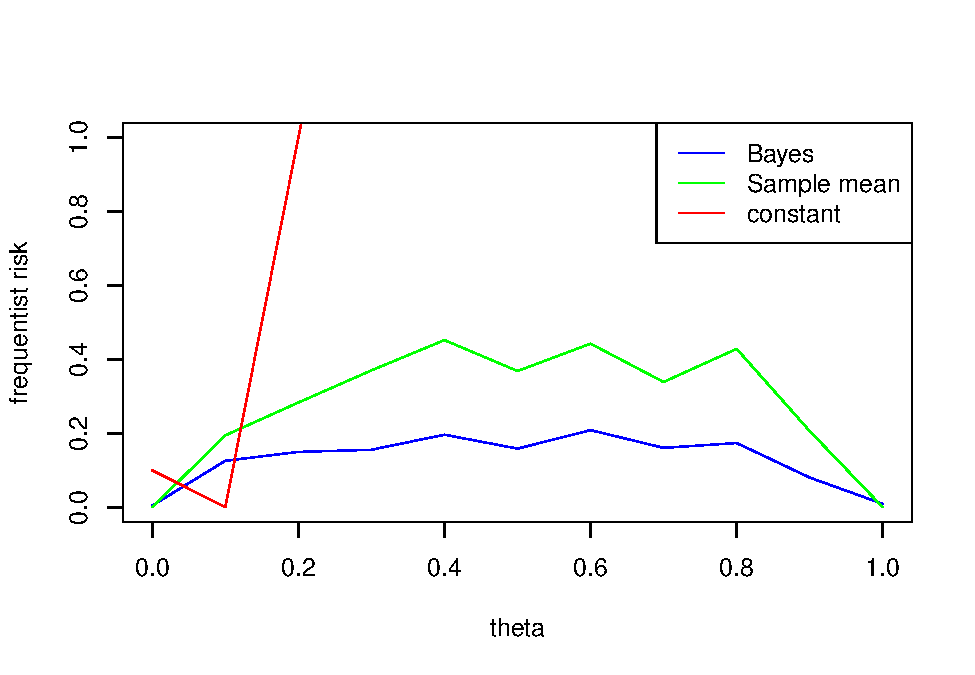
\includegraphics{lab-03_files/figure-latex/unnamed-chunk-7-1.pdf}

Please see a few remarks about Task 4 that will help you with
interpreting the plot.

\begin{enumerate}
\item If you zoom into see the plot for Task 4, you will notice that the Bayes risk is not always smaller than the sample mean. Specifically, the issue is occuring around $\theta = 0$ and $\theta = 1.$
\item One observation that we can make is that when $x$ is very small (say 0), Bayes estimator tends to overestimate $\theta$ and hence sample mean has lower risk. What other observations can you make? 
\end{enumerate}

I am including some code that Xu Chen has written that is much faster,
where the resulting plot is more clear.

\begin{Shaded}
\begin{Highlighting}[]
\CommentTok{# code by Xu Chen}
\NormalTok{loss <-}\StringTok{ }\ControlFlowTok{function}\NormalTok{(theta, c)\{}
  \ControlFlowTok{if}\NormalTok{ (c }\OperatorTok{>=}\StringTok{ }\NormalTok{theta) \{}
    \KeywordTok{return}\NormalTok{(c }\OperatorTok{-}\StringTok{ }\NormalTok{theta)}
\NormalTok{  \} }\ControlFlowTok{else}\NormalTok{ \{}
    \KeywordTok{return}\NormalTok{(}\DecValTok{10}\OperatorTok{*}\NormalTok{(theta }\OperatorTok{-}\StringTok{ }\NormalTok{c))}
\NormalTok{  \}}
\NormalTok{\}}


\NormalTok{delta1 <-}\StringTok{ }\ControlFlowTok{function}\NormalTok{(x)\{}
  \KeywordTok{return}\NormalTok{(}\KeywordTok{rep}\NormalTok{(}\FloatTok{0.1}\NormalTok{,}\KeywordTok{length}\NormalTok{(x)))}
\NormalTok{\}}


\NormalTok{delta2 <-}\StringTok{ }\ControlFlowTok{function}\NormalTok{(x)\{}
  \KeywordTok{return}\NormalTok{(x}\OperatorTok{/}\DecValTok{30}\NormalTok{)}
\NormalTok{\}}


\NormalTok{delta3 <-}\StringTok{ }\ControlFlowTok{function}\NormalTok{(x, }\DataTypeTok{a =} \FloatTok{0.05}\NormalTok{, }\DataTypeTok{b =} \DecValTok{1}\NormalTok{)\{}
\NormalTok{  a.post <-}\StringTok{ }\NormalTok{a }\OperatorTok{+}\StringTok{ }\NormalTok{x}
\NormalTok{  b.post <-}\StringTok{ }\NormalTok{b }\OperatorTok{+}\StringTok{ }\DecValTok{30} \OperatorTok{-}\StringTok{ }\NormalTok{x}
\NormalTok{  c <-}\StringTok{ }\KeywordTok{seq}\NormalTok{(}\DecValTok{0}\NormalTok{,}\DecValTok{1}\NormalTok{,}\FloatTok{0.01}\NormalTok{)}
\NormalTok{  theta <-}\StringTok{ }\KeywordTok{matrix}\NormalTok{(}\KeywordTok{rbeta}\NormalTok{(}\FloatTok{1e4}\OperatorTok{*}\KeywordTok{length}\NormalTok{(c), a.post, b.post), }
                  \DataTypeTok{nrow =} \FloatTok{1e4}\NormalTok{, }\DataTypeTok{ncol =} \KeywordTok{length}\NormalTok{(c))}
  
  \KeywordTok{return}\NormalTok{(c[}\KeywordTok{which.min}\NormalTok{(}\KeywordTok{sapply}\NormalTok{(c, }\ControlFlowTok{function}\NormalTok{(u) }\KeywordTok{mean}\NormalTok{(}\KeywordTok{sapply}\NormalTok{(theta[,}\KeywordTok{as.integer}\NormalTok{(}\DecValTok{100}\OperatorTok{*}\NormalTok{u}\OperatorTok{+}\DecValTok{1}\NormalTok{)], loss, }\DataTypeTok{c =}\NormalTok{ u))))])}
\NormalTok{\}}

\NormalTok{risk <-}\StringTok{ }\ControlFlowTok{function}\NormalTok{(theta, c)\{}
  \KeywordTok{return}\NormalTok{(}\KeywordTok{sum}\NormalTok{(}\KeywordTok{dbinom}\NormalTok{(}\DataTypeTok{x =} \DecValTok{0}\OperatorTok{:}\DecValTok{30}\NormalTok{, }\DataTypeTok{size =} \DecValTok{30}\NormalTok{, }\DataTypeTok{prob =}\NormalTok{ theta) }\OperatorTok{*}\StringTok{ }\KeywordTok{sapply}\NormalTok{(c, loss, }\DataTypeTok{theta =}\NormalTok{ theta)))}
\NormalTok{\}}


\NormalTok{theta.grid <-}\StringTok{ }\KeywordTok{seq}\NormalTok{(}\DecValTok{0}\NormalTok{,}\DecValTok{1}\NormalTok{,}\FloatTok{0.01}\NormalTok{)}
\NormalTok{x <-}\StringTok{ }\DecValTok{0}\OperatorTok{:}\DecValTok{30}

\NormalTok{c3 <-}\StringTok{ }\KeywordTok{sapply}\NormalTok{(x, delta3)}
\KeywordTok{plot}\NormalTok{(theta.grid, }\KeywordTok{sapply}\NormalTok{(theta.grid, risk, c3), }
     \DataTypeTok{ylim =} \KeywordTok{c}\NormalTok{(}\DecValTok{0}\NormalTok{,}\DecValTok{1}\NormalTok{), }\DataTypeTok{type =} \StringTok{'l'}\NormalTok{, }\DataTypeTok{col =} \StringTok{'red'}\NormalTok{, }\DataTypeTok{xlab =} \KeywordTok{expression}\NormalTok{(theta), }\DataTypeTok{ylab =} \StringTok{'risk'}\NormalTok{)}

\NormalTok{c1 <-}\StringTok{ }\KeywordTok{delta1}\NormalTok{(x)}
\KeywordTok{points}\NormalTok{(theta.grid, }\KeywordTok{sapply}\NormalTok{(theta.grid, risk, c1), }
       \DataTypeTok{ylim =} \KeywordTok{c}\NormalTok{(}\DecValTok{0}\NormalTok{,}\DecValTok{1}\NormalTok{), }\DataTypeTok{type =} \StringTok{'l'}\NormalTok{)}

\NormalTok{c2 <-}\StringTok{ }\KeywordTok{delta2}\NormalTok{(x)}
\KeywordTok{points}\NormalTok{(theta.grid, }\KeywordTok{sapply}\NormalTok{(theta.grid, risk, c2), }
       \DataTypeTok{ylim =} \KeywordTok{c}\NormalTok{(}\DecValTok{0}\NormalTok{,}\DecValTok{1}\NormalTok{), }\DataTypeTok{type =} \StringTok{'l'}\NormalTok{, }\DataTypeTok{col=}\StringTok{'green'}\NormalTok{)}

\KeywordTok{legend}\NormalTok{(}\StringTok{'topright'}\NormalTok{, }\DataTypeTok{legend =} \KeywordTok{c}\NormalTok{(}\StringTok{'Bayes'}\NormalTok{, }\StringTok{'sample mean'}\NormalTok{, }\StringTok{'constant'}\NormalTok{), }
       \DataTypeTok{col =} \KeywordTok{c}\NormalTok{(}\StringTok{'red'}\NormalTok{, }\StringTok{'green'}\NormalTok{, }\StringTok{'black'}\NormalTok{), }\DataTypeTok{lty =} \DecValTok{1}\NormalTok{)}
\end{Highlighting}
\end{Shaded}

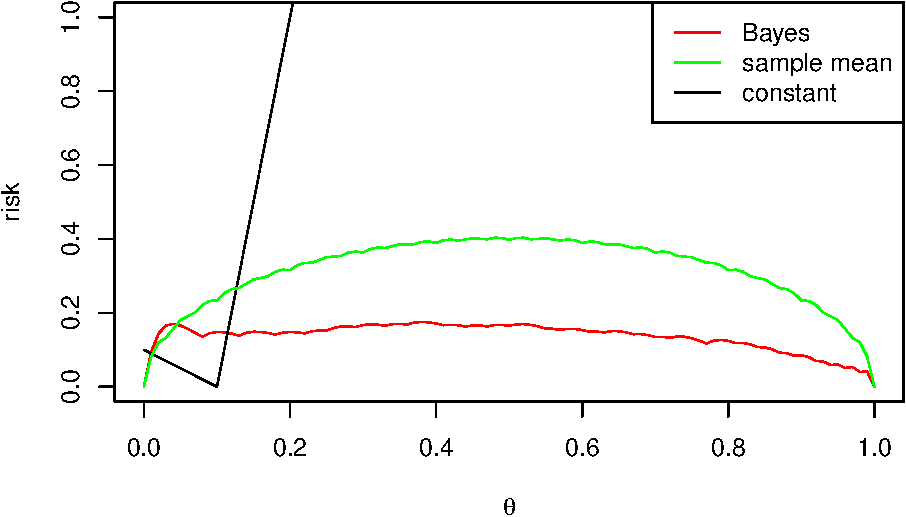
\includegraphics{lab-03_files/figure-latex/unnamed-chunk-8-1.pdf}

\hypertarget{task-5}{%
\section{Task 5}\label{task-5}}

Based on your plot of the frequentist risk, consider the three
estimators--- the constant, the mean, and the Bayes estimators. Which
estimators are admissible? Be sure to explain why or why they are not
admissible.

When \theta\$ is close to 0.1, the constant estimator has the smallest
frequentist risk among all three estimators. However, the frequentist
risk of the constant estimator increases very quickly and sharply when
\(\theta\) increases beyond 0.1.

The Bayes estimator has lower frequentist risk than the sample mean
estimator for almost all \(\theta\) values except when \(\theta\) is
close to 0 or 1.

When \(\theta\) is close to 0 or 1, sample mean estimator has lower
frequentist risk than Bayes estimator. In general, the Bayes estimator
is the best estimator for most of \(\theta\) values whereas the constant
estimator is the best estimator for \(\theta\) values close to 0.1.

Takeaway: one estimator might work better for some \(\theta\) values
whereas another estimator might work better for other \(\theta\) valuea.
Thus, all three estimators are admissible (no estimator is every
strictly better than another estimator).

\end{document}
